\chapter{ПРОЕКТИРОВАНИЕ И РЕАЛИЗАЦИЯ ВЕБ-ПРИЛОЖЕНИЯ}

\section{Архитектурное взаимодействие компонентов веб-приложения}

Проектируемая система реализуется как клиент--серверное веб-приложение. Клиентская часть отвечает за отображение пользовательского интерфейса и картографической визуализации, серверная часть --- за обработку запросов, управление данными и предоставление прикладного интерфейса~\cite{lock_aspnet_core_in_action}.

В качестве технологической основы используется следующий стек: клиентский веб-интерфейс на основе HTML, CSS, JavaScript и библиотеки Leaflet взаимодействует с серверным API на платформе ASP.NET Core по HTTP. Leaflet применяется во фронтенде для построения интерактивной карты, отображения маркеров, полилиний и полигонов, а также управления картографическими слоями. Клиент реализует представление данных, управление слоями карты и элементы управления временной шкалой, формируя параметры запросов в соответствии со сценариями использования. Серверное API обеспечивает доступ к данным, обрабатывает фильтры по времени и пространству, а также возвращает ответы в формате JSON и GeoJSON с использованием стандартных кодов HTTP.

Серверная часть обращается к базе данных через ORM Entity Framework. Использование ORM позволяет описывать схему хранения в виде классов и конфигураций, а операции выборки формировать с помощью LINQ, что снижает объём низкоуровневого SQL-кода и повышает согласованность программной модели со структурой данных. В контексте пространственных данных применяется расширение для работы с типами PostGIS, благодаря чему геометрии могут храниться и извлекаться без ручного преобразования форматов. Механизм миграций обеспечивает контролируемое изменение схемы базы данных при развитии системы и упрощает синхронизацию структуры между средами разработки и развёртывания~\cite{efcore_overview,efcore_spatial}.

Для хранения структурированных и пространственных данных применяется PostgreSQL с расширением PostGIS. Обмен данными между компонентами выполняется преимущественно в формате JSON, а пространственные объекты передаются в формате GeoJSON. Отдельно предусматривается файловое хранилище для данных, размещение которых в реляционной базе является нецелесообразным; при этом метаданные таких объектов могут храниться в базе данных и связываться с сущностями системы~\cite{postgresql_docs,postgis_manual,rfc7946}.

Общее архитектурное взаимодействие компонентов веб-приложения представлено на рисунке~\ref{fig:architecture-components}. Схема показывает связь клиентского интерфейса, серверного API, слоя доступа к данным и базы данных.

\begin{figure}[h]
    \centering
    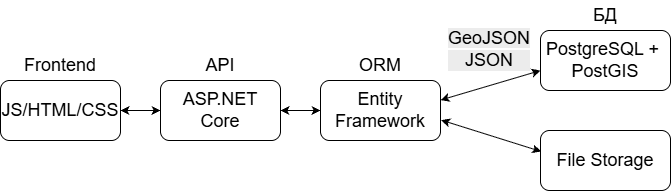
\includegraphics[width=0.95\textwidth]{../image/Stack.png}%
    \caption{Архитектурное взаимодействие компонентов веб-приложения.}
    \label{fig:architecture-components}
\end{figure}

\section{Архитектурные решения и принципы построения серверной части веб-приложения}

\subsection{Многоуровневая архитектура приложения}

Архитектура серверной части построена по многоуровневому принципу, при котором компоненты группируются по ответственности и взаимодействуют через явно определённые границы. Такой подход применяется для разделения задач представления, прикладных сценариев, предметной модели и инфраструктурных механизмов доступа к данным~\cite{sommerville2015software}. В рамках реализации выделяются следующие логические уровни:
\begin{itemize}
\item Presentation (уровень представления). Включает веб-интерфейс и серверные контроллеры API. На этом уровне выполняется приём запросов, разбор параметров и формирование ответов. Логика предметной области и операции с базой данных на уровне представления не размещаются;
\item Application (прикладной уровень). Содержит сценарии использования системы, определяющие последовательность действий для выполнения операций: получение данных на заданную дату, выборка объектов по фильтрам, формирование набора слоёв для отображения;
\item Domain (уровень предметной области). Определяет предметную область: основные сущности, их взаимосвязи и правила, которым должны соответствовать данные;
\item Infrastructure (инфраструктурный уровень). Включает механизмы работы с базой данных, реализацию репозиториев, настройку ORM и взаимодействие с файловым хранилищем.
\end{itemize}

В типовом потоке обработки пользовательский запрос поступает в контроллер API, далее управление передаётся прикладному сценарию, который использует предметные сущности и обращается к инфраструктурным интерфейсам доступа к данным. Результат преобразуется в структуру передачи данных и возвращается клиенту.

\subsection{Применение типовых архитектурных шаблонов}

Реализация серверной части опирается на типовые архитектурные шаблоны проектирования, применяемые в веб-приложениях на платформе .NET. Используемые шаблоны задают структуру взаимодействия компонентов и обеспечивают разделение ответственности между уровнями системы~\cite{fowler2002patterns,gamma1994design}.

Архитектурная модель строится на разделении компонентов по слоям: Presentation, Application, Domain и Infrastructure. Такое разграничение позволяет изолировать прикладную и предметную логику от деталей хранения данных и механизма взаимодействия по HTTP.

Компонентная структура серверной части и распределение основных элементов по слоям представлены на рисунке~\ref{fig:server-component-structure}. Данная схема используется для пояснения того, через какие уровни проходит запрос перед обращением к базе данных.

\begin{figure}[h]
    \centering
    \IfFileExists{../image/BackPattern.png}{%
        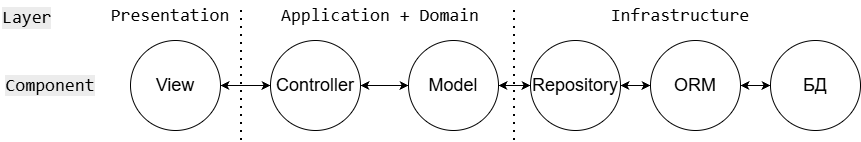
\includegraphics[width=0.95\textwidth]{../image/BackPattern.png}%
    }{%
        \fbox{\parbox[c][0.18\textheight][c]{0.9\textwidth}{\centering Временная заглушка для файла \texttt{BackPattern.png}.}}%
    }
    \caption{Компонентная структура серверной части и распределение по слоям.}
    \label{fig:server-component-structure}
\end{figure}

В рамках представленной структуры компоненты распределяются следующим образом:
\begin{itemize}
\item слой Presentation. Включает компонент View. Компонент View отвечает за формирование пользовательского интерфейса и передачу запросов к серверной части;
\item слой Application + Domain. Включает компонент Model, представляющий предметную модель системы, а также контроллеры Controller. На этом уровне располагаются сущности предметной области, их связи и правила обработки. Контроллеры принимают HTTP-запросы, выполняют их маршрутизацию, преобразование входных данных и передачу управления прикладному уровню, не выполняя прямого доступа к базе данных;
\item слой Infrastructure. Включает компоненты Repository, ORM и непосредственно базу данных. Репозитории реализуют интерфейсы доступа к данным и инкапсулируют операции выборки и сохранения. ORM Entity Framework обеспечивает отображение сущностей на реляционную структуру базы данных и формирование запросов. Хранение пространственных данных осуществляется с использованием возможностей PostGIS.
\end{itemize}

Маршрут прохождения запроса организован последовательно через указанные уровни. Пользовательское действие инициирует обращение к компоненту View, который формирует HTTP-запрос. Запрос поступает в Controller, где выполняется первичная обработка и передача управления прикладной логике. Далее обращение направляется к предметной модели, которая определяет правила выполнения операции. Для получения или изменения данных модель использует интерфейсы репозиториев. Репозиторий обращается к ORM, который формирует соответствующий запрос к базе данных. Полученный результат проходит обратный путь через слои Infrastructure, Application и Presentation и возвращается клиентской части.

Такое распределение компонентов обеспечивает:
\begin{itemize}
\item изоляцию предметной логики от механизма хранения данных;
\item независимость прикладного уровня от конкретной СУБД;
\item структурированное разграничение ответственности между уровнями;
\item возможность модификации инфраструктурных компонентов без изменения предметной модели.
\end{itemize}

MVC-подход в контексте Web API проявляется в том, что контроллеры выполняют функции уровня Presentation, принимая и обрабатывая HTTP-запросы. Модель отражает состояние предметной области и относится к уровням Application и Domain. Представление формируется на стороне клиента и также относится к уровню Presentation.

Шаблон Repository относится к инфраструктурному уровню и предоставляет унифицированный интерфейс доступа к данным. Он скрывает детали работы ORM и структуры таблиц, предоставляя прикладному уровню доступ к данным~\cite{fowler_repository}.

ORM и отображение сущностей реализуются средствами Entity Framework Core. Этот механизм обеспечивает сопоставление объектов программной модели с таблицами базы данных и отслеживание изменений сущностей. При работе с пространственными данными используются типы и функции PostGIS, что позволяет выполнять геометрические операции на уровне СУБД.

\section{Организация взаимодействия клиентской и серверной частей}

\subsection{Принципы REST-взаимодействия}

Связь между клиентской и серверной частями организуется в соответствии с архитектурным стилем REST. Сервер предоставляет набор ресурсов, соответствующих ключевым сущностям предметной области и прикладным операциям~\cite{fielding2000rest}.

Для выполнения операций используются стандартные HTTP-методы:
\begin{itemize}
\item GET --- получение наборов данных и деталей сущностей;
\item POST --- создание новых записей;
\item PUT/PATCH --- изменение существующих записей;
\item DELETE --- удаление записей.
\end{itemize}

Каждый запрос обрабатывается независимо: он содержит все данные, необходимые для выполнения операции, и не требует сохранения состояния сеанса на сервере. Для передачи данных применяется формат JSON, а для пространственных объектов --- GeoJSON. Ответы API формируются с использованием стандартных кодов состояния HTTP.

\subsection{Клиентская часть приложения и формат обмена данных}

Клиентская часть обеспечивает взаимодействие пользователя с системой: навигацию по данным, настройку отображаемых слоёв и работу с временной шкалой. Клиент формирует запросы к API и использует полученные ответы для построения визуальных представлений.

Для отображения пространственных объектов клиент получает данные в формате GeoJSON и преобразует их в элементы карты. Справочные данные и метаданные передаются в формате JSON. Связь файловых данных с сущностями системы реализуется через идентификаторы и метаданные, доступные через API~\cite{rfc7946}.

Для организации интерфейса может применяться CSS-фреймворк Bootstrap, предоставляющий набор готовых стилевых компонентов. Для картографической части фронтенда используется библиотека Leaflet, позволяющая отображать интерактивную карту, группировать пространственные объекты по слоям и обновлять их при изменении параметров запроса. Использование данных клиентских технологий рассматривается как средство ускорения разработки пользовательского интерфейса без изменения архитектурной структуры приложения.

\section{Проектирование структуры базы данных}

\subsection{Требования к БД и состав хранимой информации}

База данных веб-приложения «Палантир» является центральным компонентом системы, обеспечивающим хранение структурированной информации о военных конфликтах, их участниках, операциях, событиях и пространственных объектах. Поскольку приложение ориентировано на визуализацию данных, связанных с местом и временем, база данных должна поддерживать не только текстовые и справочные сведения, но и координаты, геометрические объекты и временные характеристики~\cite{silberschatz2019database}.

Предметная область проекта предполагает представление военных событий как пространственно-временного процесса. Поэтому в базе данных должны храниться сведения о войнах, театрах военных действий, операциях, сторонах конфликта, войсковых соединениях, событиях, положениях соединений и зонах контроля. Эти данные должны образовывать единую связанную структуру, пригодную для дальнейшей обработки серверной частью приложения.

Ключевыми требованиями к базе данных являются:
\begin{itemize}
    \item хранение структурированных и взаимосвязанных данных о конфликтах;
    \item поддержка иерархии «война --- театр военных действий --- операция»;
    \item хранение временных характеристик объектов и событий;
    \item поддержка пространственных типов для координат и зон контроля;
    \item обеспечение целостности данных с помощью первичных и внешних ключей;
    \item возможность последующего получения данных через серверное API.
\end{itemize}

Отдельное внимание должно уделяться хранению информации об участниках конфликта и войсковых соединениях. В системе необходимо различать сторону как самостоятельную сущность и её участие в конкретной войне или операции. Для соединений, в свою очередь, важно хранить не только основные сведения, но и их положение на карте в разные моменты времени~\cite{silberschatz2019database}.

С точки зрения картографической визуализации существенное значение имеют события и зоны контроля. События должны иметь дату, тип, описание и координату, а зоны контроля --- геометрию и временную привязку. Благодаря этому база данных может использоваться для отображения хода конфликта на карте и построения временной шкалы изменения обстановки~\cite{postgis_manual}.

Также необходимо учитывать, что исторические данные могут быть неполными или уточняться в процессе наполнения системы. Поэтому часть полей может допускать отсутствие значения, однако ключевые параметры, необходимые для идентификации и отображения данных, должны оставаться обязательными. Для пространственных данных важно предусмотреть и указание степени точности, поскольку положение объектов и границ в исторических источниках может быть приблизительным.

Таким образом, требования к базе данных веб-приложения «Палантир» определяются необходимостью хранения взаимосвязанных исторических, временных и пространственных данных. База данных должна обеспечивать целостное представление военных конфликтов, поддержку временной навигации, хранение геометрических объектов и возможность дальнейшего расширения структуры при развитии системы.

\subsection{Структура БД и реализация БД в PostgreSQL/PostGIS}

После определения требований к базе данных была разработана структура хранения данных для веб-приложения «Палантир». Основной задачей проектирования являлось создание такой модели, которая позволяла бы хранить сведения о военных конфликтах, их участниках, театрах военных действий, операциях, событиях, войсковых соединениях и пространственных объектах. При этом база данных должна поддерживать как реляционные связи между таблицами, так и хранение геометрических данных, необходимых для картографической визуализации.

На первоначальном этапе была сформирована логическая схема базы данных, позволившая определить основные сущности предметной области, их назначение и связи между ними. Логическая схема таблиц базы данных представлена на рисунке~\ref{fig:db-logical-schema}.

\begin{figure}[h]
    \centering
    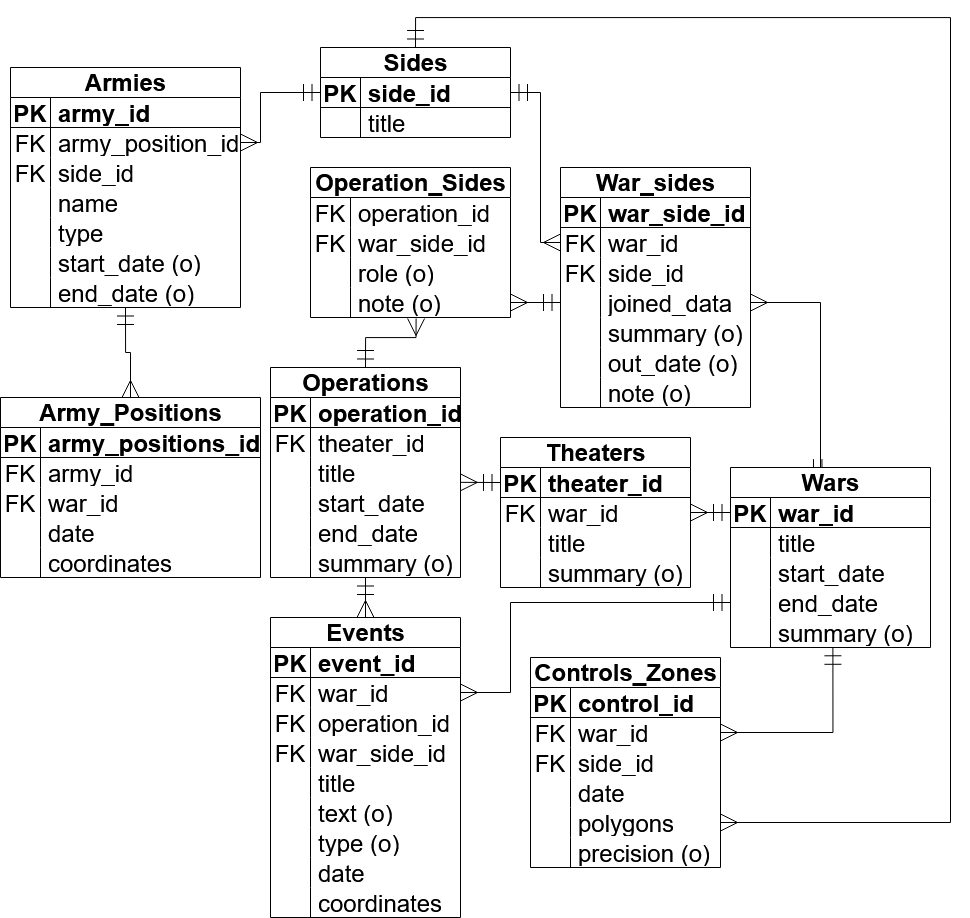
\includegraphics[width=0.72\textwidth]{../image/DB.png}
    \caption{Логическая схема таблиц базы данных веб-приложения «Палантир».}
    \label{fig:db-logical-schema}
\end{figure}

Реализация базы данных выполнена в PostgreSQL~\cite{postgresql_docs}. 
Для работы с пространственными объектами используется расширение PostGIS, которое добавляет поддержку геометрических типов данных. Это позволяет хранить не только текстовую и справочную информацию, но и координаты событий, положения войсковых соединений и полигоны зон контроля~\cite{postgis_manual}.

Использование PostGIS позволяет выполнять хранение и обработку пространственных объектов непосредственно на уровне базы данных, включая работу с точками, линиями, полигонами, пространственными индексами и запросами, применимыми в веб-картографических приложениях~\cite{obe_hsu_postgis_in_action}.

В структуре базы данных можно выделить несколько групп таблиц. Таблицы \texttt{wars}, \texttt{theaters} и \texttt{operations} задают иерархию конфликта: от войны к театрам военных действий и отдельным операциям. Таблицы \texttt{sides}, \texttt{war\_sides} и \texttt{operation\_sides} описывают участников конфликта и их роль в войнах и операциях. Таблицы \texttt{armies}, \texttt{army\_positions}, \texttt{events} и \texttt{control\_zones} содержат сведения о соединениях, их положении на карте, значимых событиях и контролируемых территориях. Такое разделение позволяет рассматривать данные как единую связанную модель и при этом сохранять логическую упорядоченность структуры~\cite{silberschatz2019database}.

Для краткого представления состава базы данных целесообразно обратиться к сводной таблице (см. таблицу~\ref{tab:db-main-tables}).

\begin{table}[H]
\caption{\label{tab:db-main-tables}Основные таблицы базы данных и их назначение}
\centering
\small
\begin{tabular}{|p{2.8cm}|p{12.2cm}|}
\hline
Таблица & Назначение \\
\hline
\texttt{wars} & Хранение общей информации о военных конфликтах \\
\hline
\texttt{theaters} & Хранение театров военных действий, относящихся к конкретной войне \\
\hline
\texttt{operations} & Хранение операций, проводимых в рамках театра военных действий \\
\hline
\texttt{sides} & Хранение справочной информации о сторонах конфликта \\
\hline
\texttt{war\_sides} & Связь сторон с конкретными войнами и хранение сведений об участии \\
\hline
\texttt{operation\_sides} & Связь сторон с конкретными операциями \\
\hline
\texttt{armies} & Хранение сведений о войсковых соединениях \\
\hline
\texttt{army\_positions} & Хранение положения соединений на карте по датам \\
\hline
\texttt{events} & Хранение событий, связанных с войной или операцией \\
\hline
\texttt{control\_zones} & Хранение зон контроля сторон конфликта \\
\hline
\end{tabular}
\end{table}

Ключевые связи в базе данных соответствуют логике предметной области. Война содержит театры военных действий, театр --- операции, а стороны конфликта связываются с войнами и операциями через промежуточные таблицы.~\cite{silberschatz2019database}.
Пространственная составляющая вынесена в таблицы \texttt{army\_positions} и \texttt{control\_zones}, что позволяет хранить изменение положения объектов и территорий во времени~\cite{postgresql_docs}. 
Полный SQL-скрипт создания базы данных приведён в приложении, а в основном тексте целесообразно показать только наиболее показательные фрагменты, один из которых представлен в листинге~\ref{code:db-key-tables}.

\begin{code}
\captionof{listing}{Фрагмент SQL-скрипта создания ключевых таблиц (полный код см. в приложении)}
\label{code:db-key-tables}
\vspace{-0.75cm}
\begin{minted}{sql}
CREATE EXTENSION IF NOT EXISTS postgis;
CREATE TABLE wars (
    war_id SERIAL PRIMARY KEY,
    title TEXT NOT NULL,
    start_date DATE NOT NULL,
    end_date DATE,
    summary TEXT
);
CREATE TABLE theaters (
    theater_id SERIAL PRIMARY KEY,
    war_id INT NOT NULL,
    title TEXT NOT NULL,
    summary TEXT,
    FOREIGN KEY (war_id) REFERENCES wars(war_id)
);
CREATE TABLE control_zones (
    control_id SERIAL PRIMARY KEY,
    war_id INT NOT NULL,
    war_side_id INT NOT NULL,
    date_control DATE NOT NULL,
    precision_control TEXT NOT NULL,
    geom geometry(MultiPolygon, 4326) NOT NULL,
    FOREIGN KEY (war_id) REFERENCES wars(war_id),
    FOREIGN KEY (war_side_id) REFERENCES war_sides(war_side_id)
);
\end{minted}
\end{code}

В приведённом фрагменте показаны базовая таблица военных конфликтов и иерархически связанная с ней таблица театров военных действий~\cite{postgresql_docs}. 
Таблица зон контроля демонстрирует использование пространственного типа \texttt{geometry(MultiPolygon, 4326)}~\cite{postgis_manual}. 
Такой набор примеров позволяет показать как реляционную структуру базы данных, так и её пространственное расширение без избыточного перечисления всех таблиц.

Для ускорения работы с данными в базе используются индексы. В контексте веб-приложения особенно важны индексы по внешним ключам, датам и геометрическим полям, поскольку они уменьшают время выборки связанных записей и ускоряют пространственные операции~\cite{postgresql_docs}. 
В качестве примера можно привести создание GiST-индекса для геометрии зон контроля, показанное в листинге~\ref{code:db-index-example}.

\begin{code}
\captionof{listing}{Пример создания пространственного индекса (полный код см. в приложении)}
\label{code:db-index-example}
\vspace{-0.75cm}
\begin{minted}{sql}
CREATE INDEX idx_control_zones_geom
    ON control_zones
    USING GIST(geom);
\end{minted}
\end{code}

Пространственный индекс ускоряет выполнение запросов к геометрическим объектам, включая выборку, фильтрацию и проверку пространственных отношений, что особенно важно для картографической визуализации данных и последующего пространственного анализа~\cite{postgis_manual}.

Таким образом, структура базы данных веб-приложения «Палантир» сочетает реляционную модель и возможности PostGIS. Она обеспечивает хранение связанных сущностей предметной области, поддержку временной навигации и работу с геометрическими объектами, создавая основу для дальнейшего доступа к данным из серверной части приложения.

\section{Реализация моделей и доступа к данным}

\subsection{Настройка Entity Framework Core и описание сущностей БД}

Для организации доступа серверной части веб-приложения «Палантир» к базе данных используется Entity Framework Core~\cite{efcore_overview}. 
Данная технология выполняет роль объектно-реляционного отображения и позволяет работать с таблицами базы данных через классы C\#, не формируя большинство SQL-запросов вручную~\cite{csharp_docs}. В рамках разрабатываемой системы это особенно важно, так как база данных содержит большое количество связанных сущностей: войны, театры военных действий, операции, стороны конфликта, армии, события и зоны контроля~\cite{smith_efcore_in_action}.

Для реализации системы была выбрана СУБД PostgreSQL с использованием расширения PostGIS, обеспечивающего поддержку пространственных типов данных. Подключение серверной части приложения к уже созданной структуре базы данных выполнено с применением подхода Database First, при котором Entity Framework Core формирует программную модель на основе существующей схемы БД~\cite{efcore_scaffolding}. 
В результате по структуре таблиц, первичным и внешним ключам, индексам и типам столбцов были получены Entity-классы базы данных, а также класс контекста \texttt{PalantirDbContext}~\cite{efcore_overview}.

Сгенерированные сущности были размещены в пространстве имён \texttt{Palantir.Domain.Models}, а сам \texttt{PalantirDbContext} --- в пространстве имён \texttt{Palantir.Infrastructure.Data}. Такой подход обеспечивает прямое соответствие между таблицами PostgreSQL/PostGIS и объектной моделью приложения. Сущности формируются на основе структуры БД и содержат свойства полей, навигационные связи и атрибуты сопоставления, автоматически отражающие схему данных~\cite{smith_efcore_in_action}.

Для системы «Палантир» важной особенностью является работа с пространственными объектами. На уровне базы данных она обеспечивается типами, предоставляемыми расширением PostGIS, а в приложении на языке C\# --- типами библиотеки NetTopologySuite~\cite{npgsql_postgis_nts}. 
Благодаря этому координаты событий, положения соединений и геометрия зон контроля единообразно представлены как в базе данных, так и в программном коде приложения~\cite{efcore_spatial}.

Центральным объектом взаимодействия с базой данных является \texttt{PalantirDbContext}. Он также был сгенерирован на основе существующей базы данных средствами Entity Framework Core и содержит наборы \texttt{DbSet}, соответствующие основным таблицам. Фрагмент данного класса приведён в листинге~\ref{code:db-context}.

\begin{code}
\captionof{listing}{Фрагмент класса \texttt{PalantirDbContext} (полный код см. в приложении)}
\label{code:db-context}
\vspace{-0.75cm}
\begin{minted}{csharp}
public partial class PalantirDbContext : DbContext {   
    public PalantirDbContext(DbContextOptions<PalantirDbContext> options) : base(options) {}
    public virtual DbSet<War> wars { get; set; }
    public virtual DbSet<Operation> operations { get; set; }
    public virtual DbSet<Event> events { get; set; }
    public virtual DbSet<ControlZone> control_zones { get; set; }
}
\end{minted}
\end{code}

Наборы \texttt{DbSet} обеспечивают доступ к таблицам базы данных через типизированные объекты и используются далее в репозиториях и сервисах приложения. Поскольку \texttt{PalantirDbContext} был сформирован по существующей структуре БД, его состав отражает актуальную схему данных и может быть расширен через механизм частичных классов без изменения сгенерированного кода напрямую~\cite{smith_efcore_in_action}.

Настройка подключения к базе данных выполняется в файле \texttt{Program.cs}, где приложение получает строку подключения из конфигурации~\cite{aspnet_configuration} и регистрирует \texttt{PalantirDbContext} в контейнере внедрения зависимостей~\cite{aspnet_docs}. Соответствующий фрагмент приведён в листинге~\ref{code:program-dbcontext}.

\begin{code}
\captionof{listing}{Регистрация контекста базы данных в \texttt{Program.cs}}
\label{code:program-dbcontext}
\vspace{-0.75cm}
\begin{minted}{csharp}
var connectionString =
    builder.Configuration.GetConnectionString(DatabaseSettings.ConnectionStringName)
    ?? throw new InvalidOperationException("Connection string not found");
builder.Services.AddDbContext<PalantirDbContext>(options =>
    options.UseNpgsql(
        connectionString,
        o => o.UseNetTopologySuite())
);
\end{minted}
\end{code}

Метод \texttt{UseNpgsql} указывает на использование PostgreSQL в качестве СУБД~\cite{npgsql_efcore_provider}. Дополнительный вызов \texttt{UseNetTopologySuite} обеспечивает корректную работу приложения с пространственными типами PostGIS, например \texttt{Point} и \texttt{MultiPolygon}~\cite{npgsql_postgis_nts}. 
В том же месте регистрируются и репозитории, через которые прикладной слой получает доступ к данным. Такая конфигурация завершает настройку компонентов доступа к базе данных и подготавливает переход к рассмотрению слоя Infrastructure.

\subsection{Реализация слоя Infrastructure для работы с БД}

Слой Infrastructure в серверной части приложения «Палантир» предназначен для реализации технических механизмов доступа к данным. В рамках данного слоя размещаются классы репозиториев, которые взаимодействуют с базой данных через \texttt{PalantirDbContext} и Entity Framework Core. За счёт этого прикладной уровень приложения не обращается к таблицам базы данных напрямую, а использует отдельные интерфейсы доступа к данным~\cite{lock_aspnet_core_in_action}.

Такой подход позволяет разделить прикладную логику и детали хранения информации. Слой Application может работать с абстракциями, не зная, каким именно образом данные извлекаются из PostgreSQL: через Entity Framework Core, SQL-запросы или иной механизм. Конкретная реализация доступа к данным находится в проекте \texttt{Palantir.Infrastructure}, а интерфейсы репозиториев вынесены в каталог \texttt{Palantir.Domain/Abstraction/Infrastructure/}. Это позволяет сохранить зависимость прикладной логики от интерфейсов, а не от конкретных инфраструктурных классов~\cite{lock_aspnet_core_in_action}.

Основным элементом слоя Infrastructure являются репозитории, отвечающие за доступ к данным по основным направлениям предметной области. Для каждой ключевой группы таблиц в проекте предусмотрены интерфейсы и их реализации, работающие через \texttt{PalantirDbContext}. Такая организация позволяет прикладному слою обращаться к данным через интерфейсы, не связывая бизнес-логику с конкретными средствами Entity Framework Core~\cite{fowler_repository}.

Репозитории имеют схожую структуру: они получают экземпляр \texttt{PalantirDbContext} через внедрение зависимостей, обращаются к соответствующим наборам \texttt{DbSet} и выполняют асинхронные операции чтения и изменения данных. В результате для прикладного слоя унифицируется работа с конфликтами, театрами военных действий, операциями, сторонами, событиями, позициями войск и зонами контроля.

Следует отметить, что интерфейсы репозиториев и классы их реализаций не относятся к автоматически сгенерированному коду Entity Framework Core. Если сущности базы данных и \texttt{PalantirDbContext} были получены на основе существующей схемы БД, то интерфейсы доступа к данным и соответствующие репозитории разрабатываются вручную. Это связано с тем, что именно они отражают выбранную архитектуру приложения и задают набор операций, доступных прикладному слою~\cite{efcore_scaffolding}.

В качестве примера можно рассмотреть интерфейс \texttt{IArmyRepository}, определяющий набор операций для работы с сущностью \texttt{Army}. Такой интерфейс фиксирует базовые операции получения, добавления, изменения и удаления данных, не раскрывая деталей конкретной реализации. Его фрагмент представлен в листинге~\ref{code:iarmy-repository}.

\begin{code}
\captionof{listing}{Интерфейс репозитория для работы с сущностью \texttt{Army}}
\label{code:iarmy-repository}
\vspace{-0.75cm}
\begin{minted}{csharp}
public interface IArmyRepository {
    Task<List<Army>> GetAllAsync();
    Task<Army?> GetByIdAsync(int id);
    Task AddAsync(Army army);
    Task UpdateAsync(Army army);
    Task DeleteAsync(int id);
}
\end{minted}
\end{code}

Наличие такого интерфейса позволяет прикладному уровню зависеть не от конкретного класса \texttt{ArmyRepository}, а от абстракции. Благодаря этому логика приложения не связывается напрямую с техническими деталями Entity Framework Core, а конкретную реализацию можно изменять без переработки кода сервисов и контроллеров~\cite{fowler_repository}.

Реализация интерфейса размещается в слое Infrastructure и использует \texttt{PalantirDbContext} для непосредственного обращения к базе данных. В отличие от Entity-классов, данный класс также создаётся разработчиком вручную и инкапсулирует конкретный способ выполнения операций над таблицей \texttt{armies}. Фрагмент реализации приведён в листинге~\ref{code:army-repository}.

\begin{code}
\captionof{listing}{Фрагмент реализации \texttt{ArmyRepository}}
\label{code:army-repository}
\vspace{-0.75cm}
\begin{minted}{csharp}
public class ArmyRepository : IArmyRepository {   
    private readonly PalantirDbContext _dbContext;
    public ArmyRepository(PalantirDbContext dbContext) {
        _dbContext = dbContext;
    }
    public async Task<List<Army>> GetAllAsync() =>
        await _dbContext.armies.ToListAsync<Army>();
    public async Task<Army?> GetByIdAsync(int id) =>
        await _dbContext.armies
            .FirstOrDefaultAsync(a => a.army_id == id);
    public async Task AddAsync(Army army) {
        await _dbContext.armies.AddAsync(army);
        await _dbContext.SaveChangesAsync();
    }
    public async Task UpdateAsync(Army army) {
        _dbContext.armies.Update(army);
        await _dbContext.SaveChangesAsync();
    }
    public async Task DeleteAsync(int id) {
        var army = await _dbContext.armies.FindAsync(id);
        if (army != null) {
            _dbContext.armies.Remove(army);
            await _dbContext.SaveChangesAsync();
        }
    }
}
\end{minted}
\end{code}

Из приведённого фрагмента видно, что класс \texttt{ArmyRepository} реализует интерфейс \texttt{IArmyRepository} и использует стандартные возможности Entity Framework Core для работы с данными. Метод \texttt{GetAllAsync} возвращает все записи из набора \texttt{armies}, \texttt{GetByIdAsync} выполняет поиск по идентификатору \texttt{army\_id}, а методы \texttt{AddAsync}, \texttt{UpdateAsync} и \texttt{DeleteAsync} изменяют данные и сохраняют результат вызовом \texttt{SaveChangesAsync}~\cite{smith_efcore_in_action}.

Отдельное значение имеют репозитории, работающие с пространственно-временными данными. При обращении к позициям войск и зонам контроля вместе с обычными атрибутами используются геометрические поля, поддерживаемые PostgreSQL/PostGIS и библиотекой NetTopologySuite~\cite{npgsql_postgis_nts}. 
По мере развития приложения такие классы могут быть дополнены методами выборки по дате, периоду времени, театру военных действий или операции, что важно для отображения исторических процессов на карте и временной шкале~\cite{efcore_spatial}.

Важной частью работы слоя Infrastructure является и его интеграция с контейнером внедрения зависимостей. Конкретные реализации репозиториев регистрируются в \texttt{Program.cs} как реализации соответствующих интерфейсов. Благодаря этому контроллеры и сервисы прикладного слоя получают зависимости через DI-контейнер, а не создают объекты репозиториев вручную. Такой способ организации соответствует многоуровневой архитектуре приложения и поддерживает изоляцию технических деталей доступа к данным внутри Infrastructure~\cite{aspnet_dependency_injection}.

Использование асинхронных методов является важной особенностью реализации репозиториев. Асинхронное выполнение операций обращения к базе данных позволяет серверному приложению эффективнее обрабатывать несколько запросов одновременно и не блокировать поток выполнения во время ожидания ответа от СУБД~\cite{csharp_docs}.

Таким образом, слой Infrastructure в проекте «Палантир» выполняет роль связующего уровня между прикладной моделью приложения и физической базой данных PostgreSQL/PostGIS. Репозитории инкапсулируют работу с Entity Framework Core и предоставляют прикладному уровню единый способ доступа к данным. В данной подглаве рассмотрены только основные и наиболее завершённые классы репозиториев, а полный исходный код реализаций и интерфейсов приведён в приложении к работе.


\subsection{Взаимодействие слоёв приложения при доступе к данным}

После настройки Entity Framework Core и описания слоя Infrastructure необходимо рассмотреть, каким образом запрос к данным проходит через уровни приложения. Для веб-приложения «Палантир» такой маршрут имеет принципиальное значение, поскольку система должна сохранять разделение ответственности между клиентским интерфейсом, серверным API, прикладной логикой, предметной моделью и механизмами хранения данных.

Типовой сценарий начинается с пользовательского действия в клиентской части. Пользователь выбирает конфликт, операцию, дату или слой карты, после чего клиентское приложение формирует HTTP-запрос к серверному API. Запрос поступает в слой Presentation, где находится API-контроллер. Контроллер отвечает за приём запроса, извлечение параметров, базовую проверку входных данных и формирование ответа, однако он не должен напрямую обращаться к таблицам базы данных или выполнять SQL-запросы. Такой подход соответствует многоуровневой архитектуре и снижает связанность между внешним интерфейсом API и техническими деталями хранения информации~\cite{lock_aspnet_core_in_action}.

После обработки входных параметров контроллер передаёт управление прикладной логике уровня Application. Данный уровень связывает пользовательский сценарий с операциями доступа к данным: например, получение списка армий, выборку событий по операции или подготовку данных для отображения на карте. При этом прикладной уровень должен зависеть не от конкретных классов Infrastructure, а от интерфейсов репозиториев. В проекте такие интерфейсы относятся к пространству имён \texttt{Palantir.Domain.Abstraction.Infrastructure}, что позволяет отделить правила предметной области и прикладные сценарии от конкретного способа работы с PostgreSQL/PostGIS.

Уровень Domain содержит сущности предметной области и абстракции, через которые остальные части приложения описывают работу с данными. К сущностям относятся модели из \texttt{Palantir.Domain.Models}, отражающие войны, операции, стороны конфликта, армии, события, позиции и зоны контроля. Уровень Infrastructure содержит реализации репозиториев, в том числе \texttt{ArmyRepository}, а также класс \texttt{PalantirDbContext}, размещённый в \texttt{Palantir.Infrastructure.Data}. Репозиторий использует \texttt{PalantirDbContext}, а контекст через Entity Framework Core и Npgsql обращается к PostgreSQL/PostGIS~\cite{npgsql_efcore_provider}.

Распределение ответственности между слоями приложения приведено в таблице~\ref{tab:data-access-layers}.

\begin{table}[H]
\caption{Распределение ролей слоёв при доступе к данным}
\label{tab:data-access-layers}
\centering
\small
\begin{tabular}{|p{2.5cm}|p{7.7cm}|p{4.8cm}|}
\hline
Слой & Назначение & Примеры компонентов \\
\hline
Presentation & Приём HTTP-запросов, извлечение параметров и формирование ответа клиентской части & API-контроллеры \\
\hline
Application & Выполнение прикладного сценария и обращение к данным через абстракции & Прикладные сценарии получения данных \\
\hline
Domain & Описание сущностей предметной области и интерфейсов доступа к данным & \texttt{Palantir.Domain.Models}, интерфейсы репозиториев \\
\hline
Infrastructure & Реализация технического доступа к базе данных и скрытие деталей хранения & \texttt{PalantirDbContext}, репозитории, \texttt{ArmyRepository} \\
\hline
\end{tabular}
\end{table}

После получения данных из базы репозиторий возвращает результат прикладному уровню. Далее данные могут быть преобразованы в DTO или response-модели, предназначенные для передачи клиентской части. Такое преобразование необходимо потому, что структура внутренней модели базы данных не всегда должна совпадать со структурой ответа API. Например, для клиентского интерфейса может быть важен только ограниченный набор полей, а для карты требуется представление пространственного объекта в формате GeoJSON~\cite{rfc7946}.

Обратный путь результата проходит через те же архитектурные границы. Infrastructure возвращает данные прикладному уровню, Application подготавливает ответ в соответствии со сценарием использования, Presentation формирует HTTP-ответ, а клиентская часть получает данные в формате JSON или GeoJSON. Таким образом, слой Infrastructure скрывает технические детали хранения данных, слой Domain задаёт сущности и абстракции, слой Application связывает пользовательские сценарии с доступом к данным, а слой Presentation выполняет роль внешней точки взаимодействия с клиентом.

Описанная схема показывает общий принцип организации доступа к данным в веб-приложении «Палантир». После рассмотрения маршрута запроса через уровни приложения целесообразно перейти к примерам запросов к базе данных через Entity Framework Core, поскольку именно они демонстрируют практический механизм получения и изменения данных в слое Infrastructure.

\subsection{Примеры запросов к БД через EF Core}

Entity Framework Core используется в серверной части приложения как основной механизм объектно-реляционного отображения. Его применение позволяет выполнять запросы к PostgreSQL через типизированные объекты C\# и выражения LINQ, не формируя большинство SQL-запросов вручную~\cite{efcore_overview}. При выполнении запроса EF Core преобразует LINQ-выражение в SQL-команду, отправляет её в СУБД через провайдер Npgsql и возвращает результат в виде объектов предметной модели.

В качестве типового примера можно рассмотреть уже приведённый в листинге~\ref{code:army-repository} фрагмент репозитория \texttt{ArmyRepository}. Метод \texttt{GetAllAsync} обращается к набору \texttt{DbSet} \texttt{armies} и получает список всех записей с помощью \texttt{ToListAsync}. Метод \texttt{GetByIdAsync} использует \texttt{FirstOrDefaultAsync} и условие по идентификатору \texttt{army\_id}. В обоих случаях запросы описываются средствами LINQ, а конкретный SQL-код формируется Entity Framework Core автоматически.

Для операций изменения данных репозиторий использует методы \texttt{AddAsync}, \texttt{Update} и \texttt{Remove}. После добавления, изменения или удаления объекта вызывается \texttt{SaveChangesAsync}, который фиксирует накопленные изменения в базе данных. Асинхронная форма этих операций позволяет серверному приложению не блокировать поток выполнения во время ожидания ответа от СУБД, что особенно важно для веб-приложения, одновременно обрабатывающего несколько HTTP-запросов~\cite{csharp_docs}.

При подготовке ответов для API данные, полученные через репозиторий, целесообразно преобразовывать в отдельные response-модели. Такой подход позволяет не возвращать клиентской части внутренние Entity-классы напрямую и контролировать структуру ответа. В качестве типового структурного примера можно рассмотреть преобразование сущности армии в краткую модель ответа, приведённое в листинге~\ref{code:army-response-example}.

\begin{code}
\captionof{listing}{Пример подготовки краткой response-модели для API}
\label{code:army-response-example}
\vspace{-0.75cm}
\begin{minted}{csharp}
var army = await armyRepository.GetByIdAsync(id);
if (army == null) {
    return null;
}
var response = new {
    Id = army.army_id,
    Title = army.title,
    Type = army.type
};
\end{minted}
\end{code}

Данный фрагмент не описывает отдельный обязательный класс проекта, а показывает общий принцип подготовки ответа: из сущности выбираются только те поля, которые необходимы клиентскому приложению. Такой подход удобен для справочных данных, отображаемых в списках, карточках объектов или панели сведений о выбранном соединении.

Для пространственно-временных данных принцип остаётся тем же, однако в запросах дополнительно учитываются дата, принадлежность к операции или стороне конфликта, а также геометрическое поле. Пространственные типы в приложении должны быть совместимы с PostGIS и NetTopologySuite, что позволяет хранить и получать точки, линии и полигоны без ручного преобразования координат~\cite{npgsql_postgis_nts}. Такая организация соответствует практическому применению пространственных типов и запросов PostGIS в веб-картографических приложениях~\cite{obe_hsu_postgis_in_action}. В качестве типового примера можно рассмотреть выборку зон контроля на заданную дату, показанную в листинге~\ref{code:control-zone-query-example}.

\begin{code}
\captionof{listing}{Типовой пример выборки пространственных данных по дате}
\label{code:control-zone-query-example}
\vspace{-0.75cm}
\begin{minted}{csharp}
var zones = await dbContext.control_zones
    .Where(zone => zone.date_control <= selectedDate)
    .ToListAsync();
\end{minted}
\end{code}

Пример демонстрирует подход к выборке объектов, связанных с временной привязкой. Полученные записи могут использоваться прикладным уровнем для подготовки ответа API, а геометрия зоны контроля --- для последующего формирования GeoJSON-структуры. В реальной реализации конкретные условия выборки могут уточняться с учётом войны, операции, стороны конфликта и требуемого временного среза.

Таким образом, запросы через Entity Framework Core позволяют связать реляционную и пространственную структуру PostgreSQL/PostGIS с объектной моделью серверного приложения. Репозитории инкапсулируют эти операции, а прикладной уровень получает данные в форме, пригодной для дальнейшей передачи через серверное API.

\section{Реализация серверного API}

Для взаимодействия клиентской части веб-приложения с серверной частью реализуется программный интерфейс API. Серверное API предназначено для приёма запросов от клиента, обработки переданных параметров, обращения к прикладной логике и возвращения данных в формате, пригодном для дальнейшего отображения в пользовательском интерфейсе~\cite{aspnet_docs}.

В рамках проекта «Палантир» API используется для работы с основными сущностями предметной области: войнами, сторонами конфликта, зонами контроля, операциями и другими объектами, связанными с отображением пространственно-временных данных. Клиентская часть отправляет HTTP-запросы к серверу, после чего сервер возвращает структурированный ответ, содержащий необходимые данные.

Для передачи данных между клиентом и сервером используются специальные классы-контракты. Они разделяются на два основных типа:
\begin{itemize}
\item \texttt{Request} --- модели входных данных, которые клиент передаёт серверу;
\item \texttt{Response} --- модели выходных данных, которые сервер возвращает клиенту.
\end{itemize}

Такое разделение позволяет не передавать клиенту внутренние сущности базы данных напрямую, а использовать отдельные структуры, предназначенные именно для обмена данными через API. Это повышает гибкость системы, упрощает сопровождение кода и позволяет изменять внутреннюю структуру базы данных без необходимости менять формат взаимодействия с клиентской частью.

Примером входной модели является класс \texttt{WarRequest}, предназначенный для передачи данных при создании или изменении записи о войне. Фрагмент модели представлен в листинге~\ref{code:war-request-api}.

\begin{code}
\captionof{listing}{Модель запроса \texttt{WarRequest}}
\label{code:war-request-api}
\vspace{-0.75cm}
\begin{minted}{csharp}
public record class WarRequest(
    string Title,
    DateOnly StartDate,
    DateOnly? EndDate,
    string? Summary
);
\end{minted}
\end{code}

Данная модель содержит название войны, дату начала, необязательную дату окончания и краткое описание. Использование типа \texttt{DateOnly} позволяет явно указать, что в данной модели важна именно календарная дата, а не точное время суток. Поля \texttt{EndDate} и \texttt{Summary} сделаны необязательными, так как для некоторых конфликтов дата окончания может быть неизвестна или описание может отсутствовать на момент создания записи.

Соответствующая модель ответа \texttt{WarResponse} дополнительно содержит идентификатор записи. Её структура приведена в листинге~\ref{code:war-response-api}.

\begin{code}
\captionof{listing}{Модель ответа \texttt{WarResponse}}
\label{code:war-response-api}
\vspace{-0.75cm}
\begin{minted}{csharp}
public record class WarResponse(
    int Id,
    string Title,
    DateOnly StartDate,
    DateOnly? EndDate,
    string? Summary
);
\end{minted}
\end{code}

Наличие поля \texttt{Id} в ответе необходимо для дальнейшего обращения к конкретной записи со стороны клиентского приложения. Например, после создания новой войны клиент может использовать полученный идентификатор для загрузки связанных с ней сторон, операций, событий или зон контроля.

Пример HTTP-запроса на создание записи о войне представлен в листинге~\ref{code:war-create-request-api}.

\begin{code}
\captionof{listing}{Пример запроса на создание записи о войне}
\label{code:war-create-request-api}
\vspace{-0.75cm}
\begin{minted}{json}
POST /api/wars
Content-Type: application/json {
  "title": "Великая Отечественная война",
  "startDate": "1941-06-22",
  "endDate": "1945-05-09",
  "summary": "Военный конфликт между СССР и странами нацистского блока в рамках Второй мировой войны."
}
\end{minted}
\end{code}

После обработки запроса сервер может вернуть ответ, приведённый в листинге~\ref{code:war-create-response-api}.

\begin{code}
\captionof{listing}{Пример ответа после создания записи о войне}
\label{code:war-create-response-api}
\vspace{-0.75cm}
\begin{minted}{http}
HTTP/1.1 201 Created
Content-Type: application/json {
  "id": 1,
  "title": "Великая Отечественная война",
  "startDate": "1941-06-22",
  "endDate": "1945-05-09",
  "summary": "Военный конфликт между СССР и странами нацистского блока в рамках Второй мировой войны."
}
\end{minted}
\end{code}

Таким образом, клиент передаёт серверу только данные, необходимые для создания записи, а сервер возвращает уже сформированный объект с присвоенным идентификатором.

Отдельное значение в системе имеют модели, связанные с зонами контроля. Зона контроля представляет собой пространственный объект, который показывает территорию, контролируемую определённой стороной конфликта на конкретную дату. Для создания такой записи используется модель \texttt{CreateControlZoneRequest}, показанная в листинге~\ref{code:create-control-zone-request-api}.

\begin{code}
\captionof{listing}{Модель запроса \texttt{CreateControlZoneRequest}}
\label{code:create-control-zone-request-api}
\vspace{-0.75cm}
\begin{minted}{csharp}
public record class CreateControlZoneRequest(
    int WarId,
    int WarSideId,
    DateOnly DateControl,
    string PrecisionControl,
    MultiPolygon Geom
);
\end{minted}
\end{code}

Данная модель содержит идентификатор войны, идентификатор стороны конфликта, дату фиксации зоны контроля, описание точности данных и геометрию объекта. Поле \texttt{Geom} имеет тип \texttt{MultiPolygon}, что позволяет хранить сложные полигональные объекты, состоящие из нескольких областей. Это важно для отображения зон контроля, так как территория, находящаяся под контролем одной стороны, может быть не сплошной, а состоять из нескольких отдельных участков~\cite{npgsql_postgis_nts}.

Поле \texttt{PrecisionControl} используется для указания степени точности пространственных данных. Например, зона контроля может быть получена на основе исторической карты, приблизительной реконструкции или другого источника, не всегда позволяющего определить границы абсолютно точно. Такое поле позволяет учитывать специфику исторических данных, где пространственная информация может иметь различную степень достоверности.

Для обновления зоны контроля используется отдельная модель \texttt{UpdateControlZoneRequest}, представленная в листинге~\ref{code:update-control-zone-request-api}.

\begin{code}
\captionof{listing}{Модель запроса \texttt{UpdateControlZoneRequest}}
\label{code:update-control-zone-request-api}
\vspace{-0.75cm}
\begin{minted}{csharp}
public record class UpdateControlZoneRequest(
    string PrecisionControl,
    MultiPolygon Geom
);
\end{minted}
\end{code}

В данной модели отсутствуют поля \texttt{WarId}, \texttt{WarSideId} и \texttt{DateControl}, так как при изменении уже существующей зоны контроля обычно корректируются именно геометрия и характеристика точности, а принадлежность к войне, стороне конфликта и дате остаётся неизменной. Это позволяет ограничить набор изменяемых данных и снизить вероятность случайного нарушения связей между сущностями.

Модель ответа для зоны контроля содержит идентификатор зоны контроля, связь с войной и стороной конфликта, дату, описание точности и геометрию. Такой ответ может использоваться клиентской частью для отображения полигона на карте. Структура модели приведена в листинге~\ref{code:control-zone-response-api}.

\begin{code}
\captionof{listing}{Модель ответа \texttt{ControlZoneResponse}}
\label{code:control-zone-response-api}
\vspace{-0.75cm}
\begin{minted}{csharp}
public record class ControlZoneResponse(
    int Id,
    int WarId,
    int WarSideId,
    DateOnly DateControl,
    string PrecisionControl,
    MultiPolygon Geom
);
\end{minted}
\end{code}

Пример запроса на создание зоны контроля представлен в листинге~\ref{code:control-zone-create-request-api}.

\begin{code}
\captionof{listing}{Пример запроса на создание зоны контроля}
\label{code:control-zone-create-request-api}
\vspace{-0.75cm}
\begin{minted}{json}
POST /api/control-zones
Content-Type: application/json {
  "warId": 1,
  "warSideId": 2,
  "dateControl": "1943-07-12",
  "precisionControl": "Граница зоны контроля построена по исторической карте и имеет приблизительный характер.",
  "geom": {
    "type": "MultiPolygon",
    "coordinates": [[[
          [36.10, 51.20],
          [36.40, 51.25],
          [36.35, 51.05],
          [36.10, 51.20]]]]}
}
\end{minted}
\end{code}

После успешного создания сервер возвращает данные созданной зоны контроля. Пример ответа приведён в листинге~\ref{code:control-zone-create-response-api}.

\begin{code}
\captionof{listing}{Пример ответа после создания зоны контроля}
\label{code:control-zone-create-response-api}
\vspace{-0.75cm}
\begin{minted}{http}
HTTP/1.1 201 Created
Content-Type: application/json {
  "id": 15,
  "warId": 1,
  "warSideId": 2,
  "dateControl": "1943-07-12",
  "precisionControl": "Граница зоны контроля построена по исторической карте и имеет приблизительный характер.",
  "geom": {
    "type": "MultiPolygon",
    "coordinates": [[[
          [36.10, 51.20],
          [36.40, 51.25],
          [36.35, 51.05],
          [36.10, 51.20]]]]}
}
\end{minted}
\end{code}

Пример изменения зоны контроля представлен в листинге~\ref{code:control-zone-update-request-api}.

\begin{code}
\captionof{listing}{Пример запроса на изменение зоны контроля}
\label{code:control-zone-update-request-api}
\vspace{-0.75cm}
\begin{minted}{json}
PUT /api/control-zones/15
Content-Type: application/json {
  "precisionControl": "Геометрия уточнена на основе дополнительного картографического источника.",
  "geom": {
    "type": "MultiPolygon",
    "coordinates": [[[
          [36.12, 51.22],
          [36.42, 51.27],
          [36.36, 51.04],
          [36.12, 51.22]]]]}
}
\end{minted}
\end{code}

В результате сервер обновляет геометрию и характеристику точности для существующей записи. Такой подход особенно важен для системы «Палантир», поскольку пространственные данные о боевых действиях могут уточняться по мере добавления новых источников.

Использование отдельных моделей запросов и ответов позволяет явно определить границы взаимодействия между клиентом и сервером. Клиентская часть не работает напрямую с таблицами базы данных, а взаимодействует с API через заранее определённые контракты. Серверная часть, в свою очередь, принимает входные данные, выполняет проверку, обращается к базе данных через слой инфраструктуры и возвращает результат в виде ответа.

Таким образом, реализация серверного API обеспечивает связь между пользовательским интерфейсом, прикладной логикой и базой данных. API выступает промежуточным уровнем, который принимает HTTP-запросы, преобразует входные данные в структуры приложения, выполняет необходимые операции и возвращает клиенту данные в унифицированном формате. Это соответствует выбранной клиент-серверной архитектуре и обеспечивает возможность дальнейшего расширения системы за счёт добавления новых маршрутов, моделей запросов и моделей ответов.
